\documentclass[twoside]{book}

% Packages required by doxygen
\usepackage{fixltx2e}
\usepackage{calc}
\usepackage{doxygen}
\usepackage[export]{adjustbox} % also loads graphicx
\usepackage{graphicx}
\usepackage[utf8]{inputenc}
\usepackage{makeidx}
\usepackage{multicol}
\usepackage{multirow}
\PassOptionsToPackage{warn}{textcomp}
\usepackage{textcomp}
\usepackage[nointegrals]{wasysym}
\usepackage[table]{xcolor}

% Font selection
\usepackage[T1]{fontenc}
\usepackage[scaled=.90]{helvet}
\usepackage{courier}
\usepackage{amssymb}
\usepackage{sectsty}
\renewcommand{\familydefault}{\sfdefault}
\allsectionsfont{%
  \fontseries{bc}\selectfont%
  \color{darkgray}%
}
\renewcommand{\DoxyLabelFont}{%
  \fontseries{bc}\selectfont%
  \color{darkgray}%
}
\newcommand{\+}{\discretionary{\mbox{\scriptsize$\hookleftarrow$}}{}{}}

% Page & text layout
\usepackage{geometry}
\geometry{%
  a4paper,%
  top=2.5cm,%
  bottom=2.5cm,%
  left=2.5cm,%
  right=2.5cm%
}
\tolerance=750
\hfuzz=15pt
\hbadness=750
\setlength{\emergencystretch}{15pt}
\setlength{\parindent}{0cm}
\setlength{\parskip}{3ex plus 2ex minus 2ex}
\makeatletter
\renewcommand{\paragraph}{%
  \@startsection{paragraph}{4}{0ex}{-1.0ex}{1.0ex}{%
    \normalfont\normalsize\bfseries\SS@parafont%
  }%
}
\renewcommand{\subparagraph}{%
  \@startsection{subparagraph}{5}{0ex}{-1.0ex}{1.0ex}{%
    \normalfont\normalsize\bfseries\SS@subparafont%
  }%
}
\makeatother

% Headers & footers
\usepackage{fancyhdr}
\pagestyle{fancyplain}
\fancyhead[LE]{\fancyplain{}{\bfseries\thepage}}
\fancyhead[CE]{\fancyplain{}{}}
\fancyhead[RE]{\fancyplain{}{\bfseries\leftmark}}
\fancyhead[LO]{\fancyplain{}{\bfseries\rightmark}}
\fancyhead[CO]{\fancyplain{}{}}
\fancyhead[RO]{\fancyplain{}{\bfseries\thepage}}
\fancyfoot[LE]{\fancyplain{}{}}
\fancyfoot[CE]{\fancyplain{}{}}
\fancyfoot[RE]{\fancyplain{}{\bfseries\scriptsize Generated by Doxygen }}
\fancyfoot[LO]{\fancyplain{}{\bfseries\scriptsize Generated by Doxygen }}
\fancyfoot[CO]{\fancyplain{}{}}
\fancyfoot[RO]{\fancyplain{}{}}
\renewcommand{\footrulewidth}{0.4pt}
\renewcommand{\chaptermark}[1]{%
  \markboth{#1}{}%
}
\renewcommand{\sectionmark}[1]{%
  \markright{\thesection\ #1}%
}

% Indices & bibliography
\usepackage{natbib}
\usepackage[titles]{tocloft}
\setcounter{tocdepth}{3}
\setcounter{secnumdepth}{5}
\makeindex

% Custom commands
\newcommand{\clearemptydoublepage}{%
  \newpage{\pagestyle{empty}\cleardoublepage}%
}

\usepackage{caption}
\captionsetup{labelsep=space,justification=centering,font={bf},singlelinecheck=off,skip=4pt,position=top}

%===== C O N T E N T S =====

\begin{document}

% Titlepage & ToC
\pagenumbering{roman}
\begin{titlepage}
\vspace*{7cm}
\begin{center}%
{\Large Object Oriented Programming Assignment 3 \\[1ex]\large 1.\+0 }\\
\vspace*{1cm}
{\large Generated by Doxygen 1.8.11}\\
\end{center}
\end{titlepage}
\clearemptydoublepage
\tableofcontents
\clearemptydoublepage
\pagenumbering{arabic}

%--- Begin generated contents ---
\chapter{Guys, for O\+OP we are creating a messaging app.}
\label{md_README}
\subsubsection*{Go through the source, ask me about any doubts.}

If I get time I will try adding other functionality to the code. I was thinking a web browser button to quickly check things mid conversation. Right now the program is functional. 
\chapter{Hierarchical Index}
\section{Class Hierarchy}
This inheritance list is sorted roughly, but not completely, alphabetically\+:\begin{DoxyCompactList}
\item \contentsline{section}{Client\+Demo}{\pageref{class_client_demo}}{}
\item \contentsline{section}{Server\+Start}{\pageref{class_server_start}}{}
\item J\+Frame\begin{DoxyCompactList}
\item \contentsline{section}{Client}{\pageref{class_client}}{}
\item \contentsline{section}{Server}{\pageref{class_server}}{}
\end{DoxyCompactList}
\end{DoxyCompactList}

\chapter{Class Index}
\section{Class List}
Here are the classes, structs, unions and interfaces with brief descriptions\+:\begin{DoxyCompactList}
\item\contentsline{section}{{\bf Client} }{\pageref{class_client}}{}
\item\contentsline{section}{{\bf Client\+Demo} }{\pageref{class_client_demo}}{}
\item\contentsline{section}{{\bf Server} }{\pageref{class_server}}{}
\item\contentsline{section}{{\bf Server\+Start} }{\pageref{class_server_start}}{}
\end{DoxyCompactList}

\chapter{Class Documentation}
\section{Client Class Reference}
\label{class_client}\index{Client@{Client}}
Inheritance diagram for Client\+:\begin{figure}[H]
\begin{center}
\leavevmode
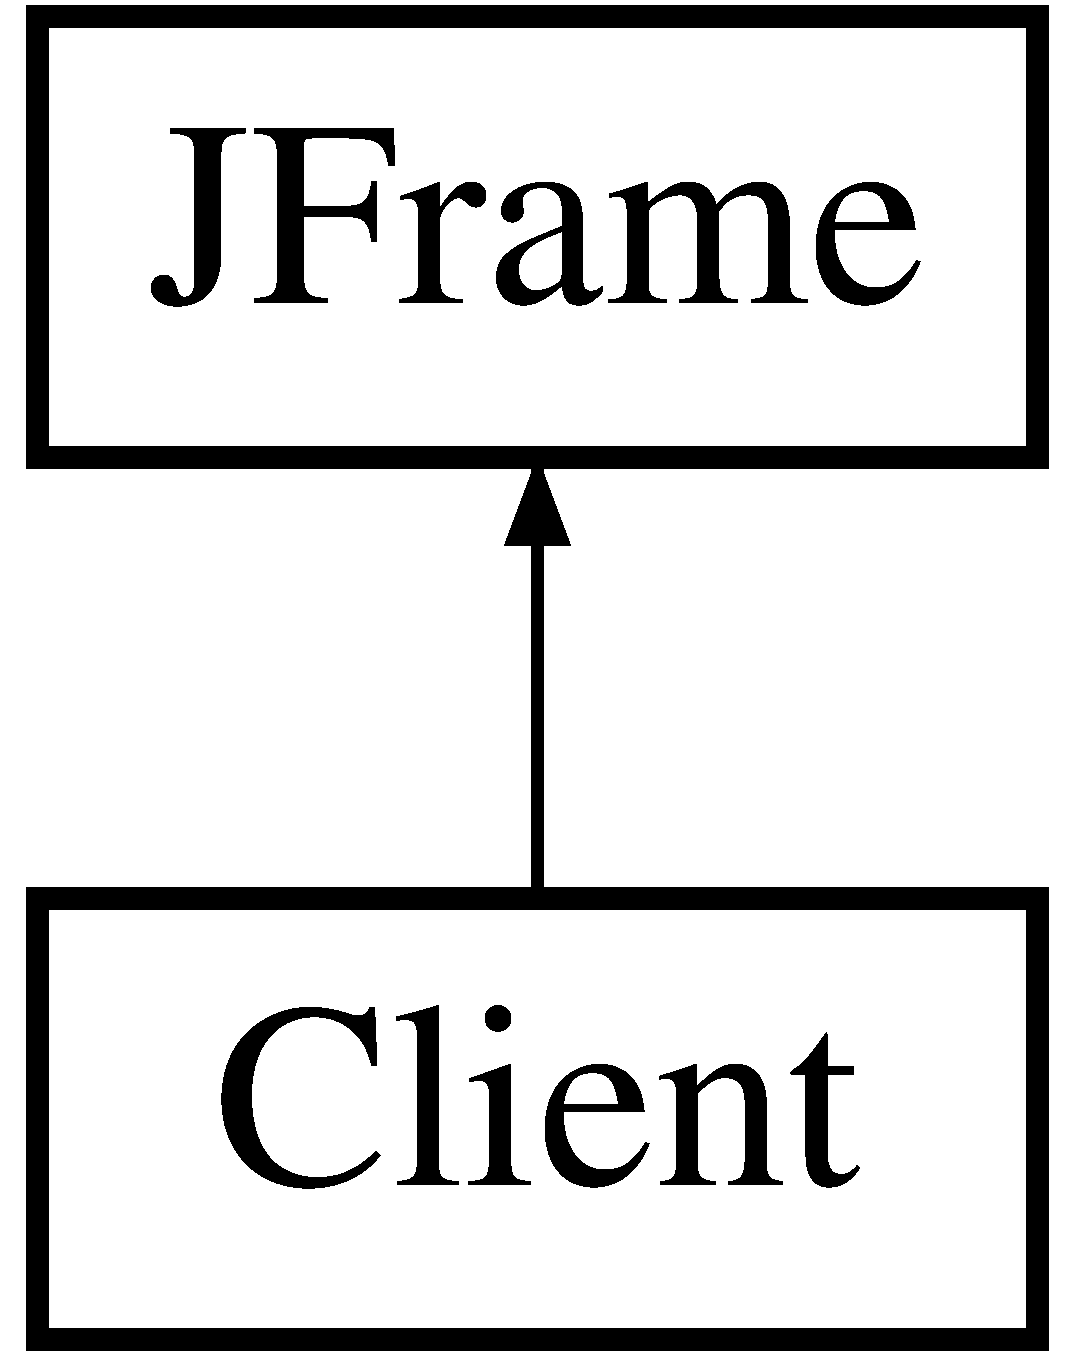
\includegraphics[height=2.000000cm]{class_client}
\end{center}
\end{figure}
\subsection*{Public Member Functions}
\begin{DoxyCompactItemize}
\item 
{\bf Client} (String host)
\item 
void {\bf begin\+Program} ()
\end{DoxyCompactItemize}
\subsection*{Private Member Functions}
\begin{DoxyCompactItemize}
\item 
void {\bf connect\+To\+Server} ()  throws I\+O\+Exception
\item 
void {\bf setup\+Streams} ()  throws I\+O\+Exception
\item 
void {\bf while\+Chatting} ()  throws I\+O\+Exception
\item 
void {\bf end\+Program} ()
\item 
void {\bf send\+Message} (String message)
\item 
void {\bf show\+Message} (final String message)
\item 
void {\bf allow\+Typing} (final boolean flag)
\item 
String {\bf format\+For\+Google} (String plain)
\end{DoxyCompactItemize}
\subsection*{Private Attributes}
\begin{DoxyCompactItemize}
\item 
J\+Text\+Field {\bfseries user\+Text}\label{class_client_aa7fe558b47954db2153276f6bd9b4924}

\item 
J\+Text\+Area {\bfseries chat\+Window}\label{class_client_a2a8bfd82dda8b8d681bea4cd90ade049}

\item 
Object\+Output\+Stream {\bfseries output}\label{class_client_a6c6fb14b922f88c0ce93e9ee8b16478b}

\item 
Object\+Input\+Stream {\bfseries input}\label{class_client_a54dd9ac6c9b61f4c74977c17b20df71d}

\item 
String {\bfseries message} = \char`\"{}\char`\"{}\label{class_client_a935da4fc44fa15fe0e20f22ccf3f6508}

\item 
String {\bfseries server\+IP}\label{class_client_af0a1fe868c66e0a184503aa551142e92}

\item 
Socket {\bfseries connection}\label{class_client_a3200b98fca84813e08d821d08ff1564f}

\item 
J\+Text\+Field {\bfseries search}\label{class_client_ab3a74bf9736f46e7bb8e0742b4ed517d}

\item 
Browser {\bfseries br}\label{class_client_a3ed0005eb086c63b69fdf4226a36fcd7}

\end{DoxyCompactItemize}


\subsection{Detailed Description}
\subsection*{The Main \doxyref{Client}{p.}{class_client} Class}

This class is called when a \doxyref{Server}{p.}{class_server} instance is launched. \begin{DoxyAuthor}{Author}
Advait Raykar, Vishwa Kalyanaraman, Parv Kapoor 
\end{DoxyAuthor}
\begin{DoxyVersion}{Version}
1.\+0 
\end{DoxyVersion}
\begin{DoxySince}{Since}
5th November 2017 
\end{DoxySince}


\subsection{Constructor \& Destructor Documentation}
\index{Client@{Client}!Client@{Client}}
\index{Client@{Client}!Client@{Client}}
\subsubsection[{Client(\+String host)}]{\setlength{\rightskip}{0pt plus 5cm}Client.\+Client (
\begin{DoxyParamCaption}
\item[{String}]{host}
\end{DoxyParamCaption}
)}\label{class_client_af140071f67f1ba90fa4c87ea536a5020}
The constructor initialises window elements, and adds the approriate event handlers. 
\begin{DoxyParams}{Parameters}
{\em host} & The host id for finding the server. \\
\hline
\end{DoxyParams}


\subsection{Member Function Documentation}
\index{Client@{Client}!allow\+Typing@{allow\+Typing}}
\index{allow\+Typing@{allow\+Typing}!Client@{Client}}
\subsubsection[{allow\+Typing(final boolean flag)}]{\setlength{\rightskip}{0pt plus 5cm}void Client.\+allow\+Typing (
\begin{DoxyParamCaption}
\item[{final boolean}]{flag}
\end{DoxyParamCaption}
)\hspace{0.3cm}{\ttfamily [private]}}\label{class_client_a2cdb479084b9154642f7010ff64a5967}
Should typing be allowed? 
\begin{DoxyParams}{Parameters}
{\em flag} & True/\+False value \\
\hline
\end{DoxyParams}
\index{Client@{Client}!begin\+Program@{begin\+Program}}
\index{begin\+Program@{begin\+Program}!Client@{Client}}
\subsubsection[{begin\+Program()}]{\setlength{\rightskip}{0pt plus 5cm}void Client.\+begin\+Program (
\begin{DoxyParamCaption}
{}
\end{DoxyParamCaption}
)}\label{class_client_aadae2d1b5b07e5cee78acc5b5d1a839e}
This method when called does the following three things\+: 
\begin{DoxyItemize}
\item Tries to connect to the server 
\item Sets up all the required streams 
\item Makes sure messages are sent and recieved properly 
\end{DoxyItemize}\index{Client@{Client}!connect\+To\+Server@{connect\+To\+Server}}
\index{connect\+To\+Server@{connect\+To\+Server}!Client@{Client}}
\subsubsection[{connect\+To\+Server()}]{\setlength{\rightskip}{0pt plus 5cm}void Client.\+connect\+To\+Server (
\begin{DoxyParamCaption}
{}
\end{DoxyParamCaption}
) throws I\+O\+Exception\hspace{0.3cm}{\ttfamily [private]}}\label{class_client_a065cf18cf33e7d6b85e5ca4f049ec7cd}
Attempts to connect to the server at P\+O\+RT 5050 which is what is used in the \doxyref{Server}{p.}{class_server} source. 
\begin{DoxyExceptions}{Exceptions}
{\em I\+O\+Exception} & \\
\hline
\end{DoxyExceptions}
\index{Client@{Client}!end\+Program@{end\+Program}}
\index{end\+Program@{end\+Program}!Client@{Client}}
\subsubsection[{end\+Program()}]{\setlength{\rightskip}{0pt plus 5cm}void Client.\+end\+Program (
\begin{DoxyParamCaption}
{}
\end{DoxyParamCaption}
)\hspace{0.3cm}{\ttfamily [private]}}\label{class_client_a10cc389ba7ae9d373df71165175b9135}
Closes all the streams after severing connections with the client. \index{Client@{Client}!format\+For\+Google@{format\+For\+Google}}
\index{format\+For\+Google@{format\+For\+Google}!Client@{Client}}
\subsubsection[{format\+For\+Google(\+String plain)}]{\setlength{\rightskip}{0pt plus 5cm}String Client.\+format\+For\+Google (
\begin{DoxyParamCaption}
\item[{String}]{plain}
\end{DoxyParamCaption}
)\hspace{0.3cm}{\ttfamily [private]}}\label{class_client_a0e4f008fda83554b408d1ad8d21ce511}
Formats the user query into a form that yeilds search results in the browser 
\begin{DoxyParams}{Parameters}
{\em plain} & The plaintext to be searched. \\
\hline
\end{DoxyParams}
\index{Client@{Client}!send\+Message@{send\+Message}}
\index{send\+Message@{send\+Message}!Client@{Client}}
\subsubsection[{send\+Message(\+String message)}]{\setlength{\rightskip}{0pt plus 5cm}void Client.\+send\+Message (
\begin{DoxyParamCaption}
\item[{String}]{message}
\end{DoxyParamCaption}
)\hspace{0.3cm}{\ttfamily [private]}}\label{class_client_a89e36eefe6212d9c47b586c616d3626f}
Sends the message to the output stream object 
\begin{DoxyParams}{Parameters}
{\em message} & This is the message that is to be sent downstream. \\
\hline
\end{DoxyParams}
\index{Client@{Client}!setup\+Streams@{setup\+Streams}}
\index{setup\+Streams@{setup\+Streams}!Client@{Client}}
\subsubsection[{setup\+Streams()}]{\setlength{\rightskip}{0pt plus 5cm}void Client.\+setup\+Streams (
\begin{DoxyParamCaption}
{}
\end{DoxyParamCaption}
) throws I\+O\+Exception\hspace{0.3cm}{\ttfamily [private]}}\label{class_client_abbd9d570746eae717ad9249001ffeee2}
Creates an
\begin{DoxyCode}
ObjectOutputStream 
\end{DoxyCode}
 object and an
\begin{DoxyCode}
ObjectInputStream 
\end{DoxyCode}
 object for sending and recieving messages 
\begin{DoxyExceptions}{Exceptions}
{\em I\+O\+Exception} & \\
\hline
\end{DoxyExceptions}
\index{Client@{Client}!show\+Message@{show\+Message}}
\index{show\+Message@{show\+Message}!Client@{Client}}
\subsubsection[{show\+Message(final String message)}]{\setlength{\rightskip}{0pt plus 5cm}void Client.\+show\+Message (
\begin{DoxyParamCaption}
\item[{final String}]{message}
\end{DoxyParamCaption}
)\hspace{0.3cm}{\ttfamily [private]}}\label{class_client_af09a9786911bb703ad17f5e9df41a604}
This prints out the message on the chat window so it\textquotesingle{}s visible to the user. 
\begin{DoxyParams}{Parameters}
{\em text} & The text to be displayed \\
\hline
\end{DoxyParams}
\index{Client@{Client}!while\+Chatting@{while\+Chatting}}
\index{while\+Chatting@{while\+Chatting}!Client@{Client}}
\subsubsection[{while\+Chatting()}]{\setlength{\rightskip}{0pt plus 5cm}void Client.\+while\+Chatting (
\begin{DoxyParamCaption}
{}
\end{DoxyParamCaption}
) throws I\+O\+Exception\hspace{0.3cm}{\ttfamily [private]}}\label{class_client_a0b594a6d81175640a2655cfde594cdf2}
Manages calls to
\begin{DoxyCode}
showMessage() 
\end{DoxyCode}
 Note, the prgram quits connection when user inputs {\itshape  xoxo } which is slang for {\itshape  \textquotesingle{}hearts and kisses\textquotesingle{} } 
\begin{DoxyExceptions}{Exceptions}
{\em I\+O\+Exception} & \\
\hline
\end{DoxyExceptions}


The documentation for this class was generated from the following file\+:\begin{DoxyCompactItemize}
\item 
Client.\+java\end{DoxyCompactItemize}

\section{Client\+Demo Class Reference}
\label{class_client_demo}\index{Client\+Demo@{Client\+Demo}}
\subsection*{Static Public Member Functions}
\begin{DoxyCompactItemize}
\item 
static void {\bfseries main} (String[$\,$] args)\label{class_client_demo_a523612ad01c2dab05b7cb9938451924a}

\end{DoxyCompactItemize}


\subsection{Detailed Description}
\subsection*{The class that calls the \doxyref{Client}{p.}{class_client} class.}

Instantiates the \doxyref{Client}{p.}{class_client} class object and starts the \doxyref{Client}{p.}{class_client}. The host passed in the constructor is ip of the localhost, so that the program can run locally. This can be changed per convience. \begin{DoxyAuthor}{Author}
Advait Raykar, Vishwa Kalyanaraman, Parv Kapoor 
\end{DoxyAuthor}
\begin{DoxyVersion}{Version}
1.\+0 
\end{DoxyVersion}
\begin{DoxySince}{Since}
5th November 2017 
\end{DoxySince}


The documentation for this class was generated from the following file\+:\begin{DoxyCompactItemize}
\item 
Client\+Demo.\+java\end{DoxyCompactItemize}

\section{Server Class Reference}
\label{class_server}\index{Server@{Server}}
Inheritance diagram for Server\+:\begin{figure}[H]
\begin{center}
\leavevmode
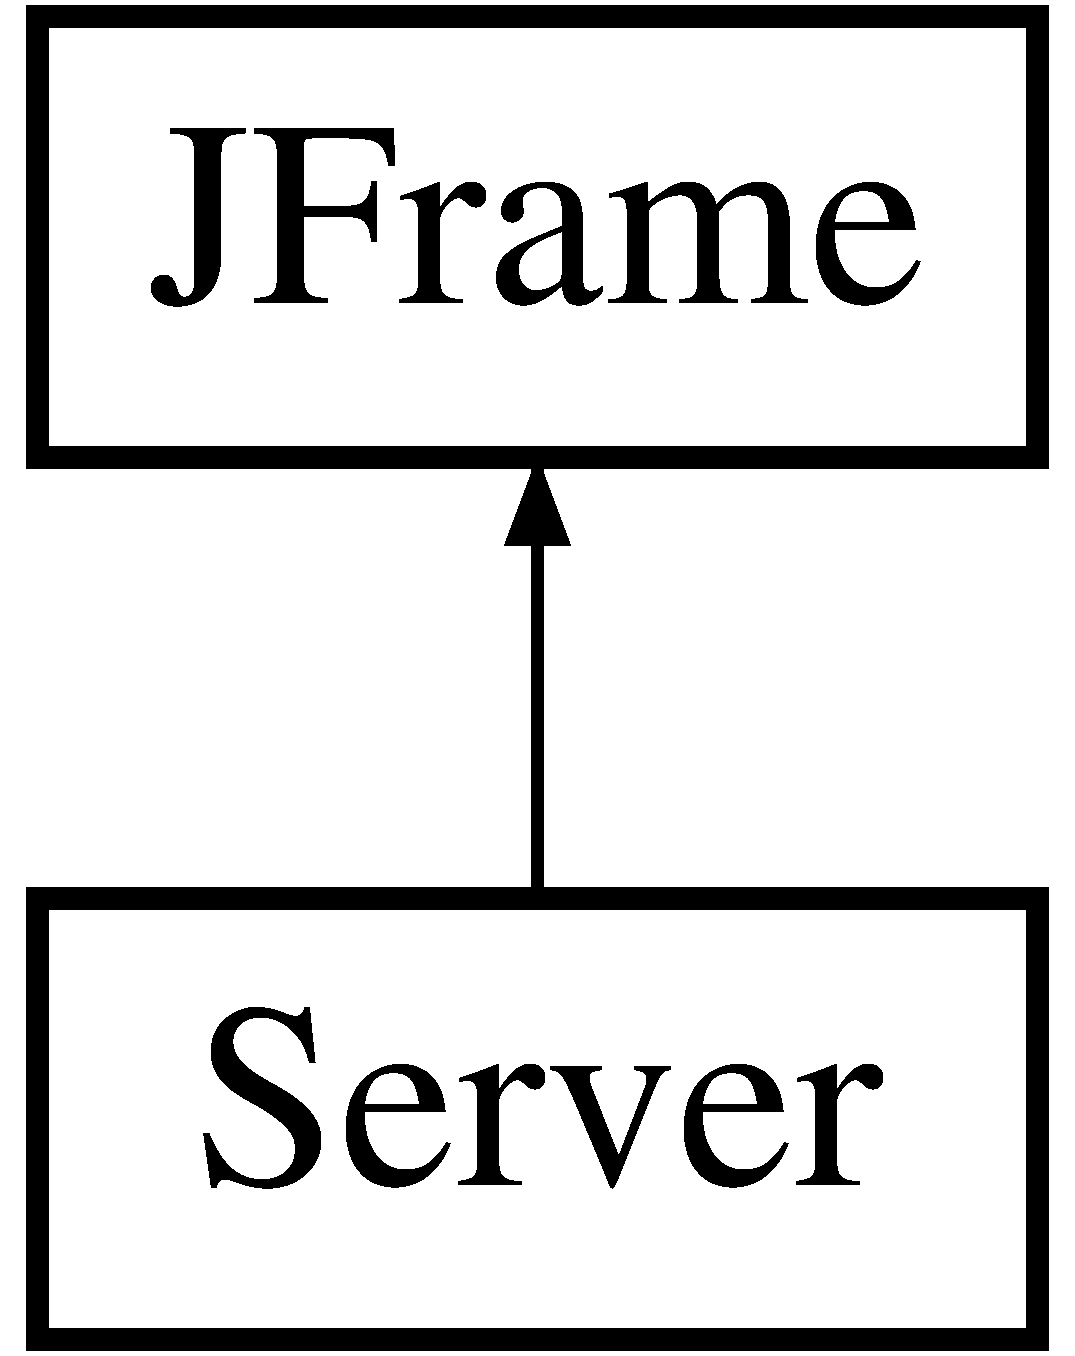
\includegraphics[height=2.000000cm]{class_server}
\end{center}
\end{figure}
\subsection*{Public Member Functions}
\begin{DoxyCompactItemize}
\item 
{\bf Server} ()
\item 
void {\bf begin\+Program} ()
\end{DoxyCompactItemize}
\subsection*{Private Member Functions}
\begin{DoxyCompactItemize}
\item 
void {\bf wait\+For\+Connection} ()  throws I\+O\+Exception
\item 
void {\bf setup\+Streams} ()  throws I\+O\+Exception
\item 
void {\bf while\+Chatting} ()  throws I\+O\+Exception
\item 
void {\bf end\+Program} ()
\item 
void {\bf send\+Message} (String message)
\item 
void {\bf show\+Message} (final String text)
\item 
void {\bf allow\+Typing} (final boolean flag)
\item 
String {\bf format\+For\+Google} (String plain)
\end{DoxyCompactItemize}
\subsection*{Private Attributes}
\begin{DoxyCompactItemize}
\item 
J\+Text\+Field {\bfseries user\+Text}\label{class_server_abf4d769d3d5587c9c441584cb1b39072}

\item 
J\+Text\+Area {\bfseries chat\+Window}\label{class_server_aec39cc324f8dba244a8f1997577ad24b}

\item 
Object\+Output\+Stream {\bfseries output}\label{class_server_a3ee83f3537ecb91aaa128c67a666197e}

\item 
Object\+Input\+Stream {\bfseries input}\label{class_server_ab08c327e4eb98bfcc9e99322ab95e962}

\item 
J\+Text\+Field {\bfseries search}\label{class_server_a09e54dd47266f5d46b8726440fcb3d06}

\item 
Browser {\bfseries br}\label{class_server_a54ffafdfbaccc84064973e51381c18cb}

\item 
Server\+Socket {\bfseries server}\label{class_server_a24129ae964202c8df4ecccdb97080b0c}

\item 
Socket {\bfseries connection}\label{class_server_acecb2d29750ac0ac276a90fab96a84ab}

\end{DoxyCompactItemize}


\subsection{Detailed Description}
\subsection*{The Main \doxyref{Server}{p.}{class_server} Class}

This class is called when a \doxyref{Server}{p.}{class_server} instance is launched. \begin{DoxyAuthor}{Author}
Advait Raykar, Vishwa Kalyanaraman, Parv Kapoor 
\end{DoxyAuthor}
\begin{DoxyVersion}{Version}
1.\+0 
\end{DoxyVersion}
\begin{DoxySince}{Since}
5th November 2017 
\end{DoxySince}


\subsection{Constructor \& Destructor Documentation}
\index{Server@{Server}!Server@{Server}}
\index{Server@{Server}!Server@{Server}}
\subsubsection[{Server()}]{\setlength{\rightskip}{0pt plus 5cm}Server.\+Server (
\begin{DoxyParamCaption}
{}
\end{DoxyParamCaption}
)}\label{class_server_a0523b403c83475114d3be0143f3321ad}
This is the constructor, which intialises the actual window, adds the necessary action listners, and adds the swing elements to the window. 

\subsection{Member Function Documentation}
\index{Server@{Server}!allow\+Typing@{allow\+Typing}}
\index{allow\+Typing@{allow\+Typing}!Server@{Server}}
\subsubsection[{allow\+Typing(final boolean flag)}]{\setlength{\rightskip}{0pt plus 5cm}void Server.\+allow\+Typing (
\begin{DoxyParamCaption}
\item[{final boolean}]{flag}
\end{DoxyParamCaption}
)\hspace{0.3cm}{\ttfamily [private]}}\label{class_server_a37ff153817bab08ab4a9c91aa9f9848f}
Should typing be allowed? 
\begin{DoxyParams}{Parameters}
{\em flag} & True/\+False value \\
\hline
\end{DoxyParams}
\index{Server@{Server}!begin\+Program@{begin\+Program}}
\index{begin\+Program@{begin\+Program}!Server@{Server}}
\subsubsection[{begin\+Program()}]{\setlength{\rightskip}{0pt plus 5cm}void Server.\+begin\+Program (
\begin{DoxyParamCaption}
{}
\end{DoxyParamCaption}
)}\label{class_server_ad3059b8fec91bbc05bf9c9bbcfd2e880}
This method when called does the following three things\+: 
\begin{DoxyItemize}
\item Waits for a client to connect 
\item Sets up all the required streams 
\item Makes sure messages are sent and recieved properly 
\end{DoxyItemize}\index{Server@{Server}!end\+Program@{end\+Program}}
\index{end\+Program@{end\+Program}!Server@{Server}}
\subsubsection[{end\+Program()}]{\setlength{\rightskip}{0pt plus 5cm}void Server.\+end\+Program (
\begin{DoxyParamCaption}
{}
\end{DoxyParamCaption}
)\hspace{0.3cm}{\ttfamily [private]}}\label{class_server_a6c370d3eb9fa4b5d9805c451da3fc49c}
Closes all the streams after severing connections with the client. \index{Server@{Server}!format\+For\+Google@{format\+For\+Google}}
\index{format\+For\+Google@{format\+For\+Google}!Server@{Server}}
\subsubsection[{format\+For\+Google(\+String plain)}]{\setlength{\rightskip}{0pt plus 5cm}String Server.\+format\+For\+Google (
\begin{DoxyParamCaption}
\item[{String}]{plain}
\end{DoxyParamCaption}
)\hspace{0.3cm}{\ttfamily [private]}}\label{class_server_aad9c759285859f7ce8bcd6ad6f020e35}
Formats the user query into a form that yeilds search results in the browser 
\begin{DoxyParams}{Parameters}
{\em plain} & The plaintext to be searched. \\
\hline
\end{DoxyParams}
\index{Server@{Server}!send\+Message@{send\+Message}}
\index{send\+Message@{send\+Message}!Server@{Server}}
\subsubsection[{send\+Message(\+String message)}]{\setlength{\rightskip}{0pt plus 5cm}void Server.\+send\+Message (
\begin{DoxyParamCaption}
\item[{String}]{message}
\end{DoxyParamCaption}
)\hspace{0.3cm}{\ttfamily [private]}}\label{class_server_a24de04f64d373247d2ab1fdfe2477dc8}
Sends the message to the output stream object 
\begin{DoxyParams}{Parameters}
{\em message} & This is the message that is to be sent downstream. \\
\hline
\end{DoxyParams}
\index{Server@{Server}!setup\+Streams@{setup\+Streams}}
\index{setup\+Streams@{setup\+Streams}!Server@{Server}}
\subsubsection[{setup\+Streams()}]{\setlength{\rightskip}{0pt plus 5cm}void Server.\+setup\+Streams (
\begin{DoxyParamCaption}
{}
\end{DoxyParamCaption}
) throws I\+O\+Exception\hspace{0.3cm}{\ttfamily [private]}}\label{class_server_a2daa10694033f06fa97d1f62129dccce}
Creates an
\begin{DoxyCode}
ObjectOutputStream 
\end{DoxyCode}
 object and an
\begin{DoxyCode}
ObjectInputStream 
\end{DoxyCode}
 object for sending and recieving messages 
\begin{DoxyExceptions}{Exceptions}
{\em I\+O\+Exception} & \\
\hline
\end{DoxyExceptions}
\index{Server@{Server}!show\+Message@{show\+Message}}
\index{show\+Message@{show\+Message}!Server@{Server}}
\subsubsection[{show\+Message(final String text)}]{\setlength{\rightskip}{0pt plus 5cm}void Server.\+show\+Message (
\begin{DoxyParamCaption}
\item[{final String}]{text}
\end{DoxyParamCaption}
)\hspace{0.3cm}{\ttfamily [private]}}\label{class_server_a10e393183360a25f9687448e4bdddd44}
This prints out the message on the chat window so it\textquotesingle{}s visible to the user. 
\begin{DoxyParams}{Parameters}
{\em text} & The text to be displayed \\
\hline
\end{DoxyParams}
\index{Server@{Server}!wait\+For\+Connection@{wait\+For\+Connection}}
\index{wait\+For\+Connection@{wait\+For\+Connection}!Server@{Server}}
\subsubsection[{wait\+For\+Connection()}]{\setlength{\rightskip}{0pt plus 5cm}void Server.\+wait\+For\+Connection (
\begin{DoxyParamCaption}
{}
\end{DoxyParamCaption}
) throws I\+O\+Exception\hspace{0.3cm}{\ttfamily [private]}}\label{class_server_a7e5f40ab891af8ed2a0e0a1ccee85397}
Waits for connection on starting the server. 
\begin{DoxyExceptions}{Exceptions}
{\em I\+O\+Exception} & \\
\hline
\end{DoxyExceptions}
\index{Server@{Server}!while\+Chatting@{while\+Chatting}}
\index{while\+Chatting@{while\+Chatting}!Server@{Server}}
\subsubsection[{while\+Chatting()}]{\setlength{\rightskip}{0pt plus 5cm}void Server.\+while\+Chatting (
\begin{DoxyParamCaption}
{}
\end{DoxyParamCaption}
) throws I\+O\+Exception\hspace{0.3cm}{\ttfamily [private]}}\label{class_server_a555be7f59ba6ca27e964e42f07cdf23e}
Manages calls to
\begin{DoxyCode}
showMessage() 
\end{DoxyCode}
 Note, the prgram quits connection when user inputs {\itshape  xoxo } which is slang for {\itshape  \textquotesingle{}hearts and kisses\textquotesingle{} } 
\begin{DoxyExceptions}{Exceptions}
{\em I\+O\+Exception} & \\
\hline
\end{DoxyExceptions}


The documentation for this class was generated from the following file\+:\begin{DoxyCompactItemize}
\item 
Server.\+java\end{DoxyCompactItemize}

\section{Server\+Start Class Reference}
\label{class_server_start}\index{Server\+Start@{Server\+Start}}
\subsection*{Static Public Member Functions}
\begin{DoxyCompactItemize}
\item 
static void {\bfseries main} (String[$\,$] args)\label{class_server_start_a80bb66ebec03efd252cfb82d9f1f98d7}

\end{DoxyCompactItemize}


\subsection{Detailed Description}
\subsection*{The class that calls the \doxyref{Server}{p.}{class_server} class.}

Instantiates the \doxyref{Server}{p.}{class_server} class object and starts the server. \begin{DoxyAuthor}{Author}
Advait Raykar, Vishwa Kalyanaraman, Parv Kapoor 
\end{DoxyAuthor}
\begin{DoxyVersion}{Version}
1.\+0 
\end{DoxyVersion}
\begin{DoxySince}{Since}
5th November 2017 
\end{DoxySince}


The documentation for this class was generated from the following file\+:\begin{DoxyCompactItemize}
\item 
Server\+Start.\+java\end{DoxyCompactItemize}

%--- End generated contents ---

% Index
\backmatter
\newpage
\phantomsection
\clearemptydoublepage
\addcontentsline{toc}{chapter}{Index}
\printindex

\end{document}
